\documentclass[a4paper]{article}
\usepackage[francais]{babel}
\usepackage[T1]{fontenc}
\usepackage[utf8]{inputenc}
\usepackage[figbotcap]{subfigure}  % use for side-by-side figures - ver  http://linuxdicas.wikispaces.com/latex
\usepackage{graphicx,amsmath,amssymb,algorithmic,algorithm,url,hyperref,tikz,exam}
\usepackage[babel=true,kerning=true]{microtype} % <- bug labels tikz
\usetikzlibrary{arrows,shapes,snakes,automata,backgrounds,petri}

\graphicspath{{./},{../figures/},{../figures/automates/}}

\newtheorem{definition}{Définition}

\paper{IN310}
\school{ISAE - Supaero}
\subject{EXAMEN}
\title{Modèles de Systèmes Embarqués : modèles discrets, modèles hybrides}
\semester{3A SEM}
\year{2010-2011}
\note{Documents interdits. Des rappels de cours sont donnés à la fin de chaque partie.}

\begin{document}

%%%%%%%%%%%%%%%%%%%%%%%%%%%%%%%%%%%%%%%%%%
%%%%%%%%%%%% RESEAUX DE PETRI %%%%%%%%%%%%
%%%%%%%%%%%%%%%%%%%%%%%%%%%%%%%%%%%%%%%%%%

\exercice{Réseaux de Petri}

On modélise par le réseau de Petri de la figure \ref{petri} le fonctionnement d'un atelier qui doit réaliser deux types de pièces.
Pour le premier type de pièce, un opérateur doit placer la pièce dans une machine puis la retirer quand la machine a fini son travail.
Le deuxième type de pièce est traité de façon manuelle par un des deux opérateurs.

\begin{figure}[!h]
\begin{center}
	\begin{tikzpicture}[node distance=1.3cm,>=stealth',bend angle=45,auto]
	\tikzstyle{place}=[circle,thick,draw=blue!75,fill=blue!20,minimum size=6mm]
  	\tikzstyle{transition}=[rectangle,thick,draw=black!75,fill=black!20,minimum size=4mm]

    \node [transition] (t1) [label=above:$t_1$] {};
    \node [place] (p1) [below of=t1,label=left:$p_1$] {};
    \node [transition] (t2) [below of=p1,label=right:$t_2$] {};
    \node [place] (p2) [below of=t2,label=left:$p_2$] {};
    \node [transition] (t3) [below of=p2,label=right:$t_3$] {};
    \node [place] (p3) [below of=t3,label=left:$p_3$] {};
    \node [transition] (t4) [below of=p3,label=left:$t_4$] {};
    \node [place,tokens=1] (p4) [left of=p2,label=left:$p_4$] {};
    \node [place,tokens=2] (p5) [right of=p1,label=left:$p_5$] {};
    \node [place] (p6) [right of=p5,label=right:$p_6$] {};
    \node [transition] (t5) [above of=p6,label=right:$t_5$] {};
    \node [transition] (t6) [below of=p6,label=right:$t_6$] {};

	\draw (t1)
		edge [pre,bend left] (p5)
		edge [post] (p1);
	\draw (t2)
		edge [pre] (p1)
		edge [pre,bend right] (p4)
		edge [post] (p2)
		edge [post,bend right] (p5);
	\draw (t3)
		edge [pre] (p2)
		edge [pre] (p5)
		edge [post] (p3)
		edge [post,bend left] (p4);
	\draw (t4)
		edge [pre] (p3)
		edge [post,bend right] (p5);
	\draw (t5)
		edge [pre,bend right] (p5)
		edge [post] (p6);
	\draw (t6)
		edge [pre] (p6)
		edge [post,bend left] (p5);
	\end{tikzpicture}
	\caption{Réseau de Petri de l'atelier.}
	\label{petri}
\end{center}
\end{figure}

\begin{questions}
\question Donner la définition du réseau $R$ de la figure \ref{petri} ($P$, $T$, $Pre$ et $Post$) et son marquage initial $M_0$.
\question Donner la signification des six places du réseau $R$.
\question Etudier les propriétés du réseau $R$ :
	\begin{enumerate}
	\item $R$ est-il borné ? Si oui, donner la valeur de la borne ;
	\item $R$ est-il vivant ?
	\item $R$ est-il ré-initialisable ?
	\end{enumerate}
\question Trouver au moins deux invariants de place du réseau. Que représentent-t-ils ?
\end{questions}

\subsection*{Rappels de cours}

Soit $R = <P, T, Pre, Post>$ un réseau de Petri, $M_0$ son marquage initial, et $A$ l'ensembe des marquages accessibles de $R$ depuis $M_0$.

\begin{definition}[Réseau borné]
$R$ est borné si et seulement si $\exists k \in \mathbb{N}$ tel que $\forall M \in A$, $\forall p \in P$, $M(p) \leq k$.
\end{definition}

\begin{definition}[Réseau vivant]
$R$ est vivant si et seulement si $\forall t \in T$, $\forall M \in A$, il existe une séquence de tir $s$ et un marquage $M' \in A$ tels que
$M \overset{st}{\longrightarrow} M'$.
\end{definition}

\begin{definition}[Réseau réinitialisable]
$R$ est réinitialisable si et seulement si $\forall M \in A$, il existe une séquence de tir $s$ telle que 
$M \overset{s}{\longrightarrow} M_0$.
\end{definition}

\begin{definition}[Composante conservative]
Une composante conservative de $R$ est une combinaison linéaire des marquages des places du réseau, représentée par une vecteur $f$, 
telle que $\forall M \in A$, $f.M = f.M_0$.
\end{definition}

%%%%%%%%%%%%%%%%%%%%%%%%%%%%%%%%%%%%%%%%%%
%%%%%%%%%%%% AUTOMATES %%%%%%%%%%%%%%%%%%%
%%%%%%%%%%%%%%%%%%%%%%%%%%%%%%%%%%%%%%%%%%

\exercice{Automates}

\begin{questions}
\question \textbf{Équivalence pour des systèmes : } Rappeler, à l'aide d'un exemple, en quoi l'équivalence de traces n'est
	pas toujours suffisante pour comparer deux systèmes.\\
	\emph{Réponse de 5 lignes maximum + un dessin éventuellement}
\question \textbf{Automates temporisés : } Considérons l'automate temporisé de la figure \ref{automateT} sur l'alphabet (ensemble de labels)
	$\Sigma=\{a_1,a_2,a_3\}$, comportant une horloge $x$. Donner, sans justification,  deux exemples de traces temporisées reconnues par cet
	automate. (Donner des séquences sur $\Sigma \times \mathbb{R}_+$, c'est à dire des séquences de paires (\texttt{label}, 
	\texttt{durée d'attente})).
	\begin{figure}[!h]
		\begin{center}
		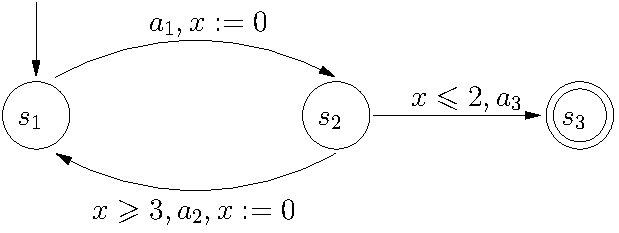
\includegraphics[width=6cm]{automate_temp}
		\end{center}
		\caption{Automate temporisé.}
		\label{automateT}
	\end{figure}
\question La sémantique d'un automate temporisé est donnée par un système de transitions temporisé, dont l'espace d'état est infini.
	Rappeler les grandes idées de la construction d'un système de transitions fini (qui permet donc de vérifier certaines propriétés)
	<<équivalent>> au système de transition temporisé infini. Dans quel sens est-il équivalent?\\
	\emph{Réponse de 10 lignes maximum }
\question Soient $T=(S,S_I,S_F,\rhd )$ et $T'=(S',S'_I,S'_F,\rhd')$ deux systèmes de transitions temporisés. Si $\mathcal{R}$ est une
	relation de bisimulation temps-abstraite qui respecte l'état initial et l'état final montrer que Untime(L(T))=Untime(L(T')).
\end{questions}

\subsection*{Rappels de cours}
\begin{definition}[Système de transitions temporisé]
Un système de transition temporisé sur un alphabet $\Sigma$ est un quadruplet
$T=(S,S_I,S_F,\rhd)$, où
\begin{itemize}
\item $S$ est l'ensemble des états
\item $S_I \subseteq S$ (resp. $S_F\subseteq S$) est l'ensemble des états initiaux (resp. finaux)
\item $\rhd \subseteq S \times (\mathbb{R}_+ \times \Sigma) \times S$
  est la fonction de transition, $s_1 \overset{t,a}{\rhd}s_2$ exprime
  qu'on peut passer de l'état $s_1$ à l'état $s_2$, en reconnaissant
  le label $a\in \Sigma$, après avoir attendu $t\in \mathbb{R}^+$
  unités de temps.
\end{itemize} 
\end{definition}

\begin{definition}[Bisimulation temps-abstraite]
Soient $T=(S,S_I,S_F,\rhd)$ et $T'=(S',S_I',S_F',\rhd')$ deux systèmes
de transitions temporisés sur $\Sigma$.
$\mathcal{R} \subseteq S\times S'$ est une relation de bisimulation
temps-abstraite ssi elle est \textbf{symétrique} et :

\begin{tabular}{ll}
 si &$(s_1,s_1')\in \mathcal{R}$ et $s_1 \overset{t,a}{\rhd}s_2$ alors
  $\exists s_2'\in S' \ \exists t'\in \mathbb{R}_+$ tels que\\
  &$(s_2,s_2')\in \mathcal{R}$ et $s_1'\overset{t',a}{\rhd}s_2'$\\
\end{tabular}

On dit que $\mathcal{R}$ \textbf{respecte les états initiaux} (resp. \textbf{finaux}) si \\
$
\begin{array}{llcl}
\forall s\in S & s\in S_I (\text{resp.} S_F)& \quad \text{si et
  seulement si} \quad & \exists s'\in S_I' (\text{resp.} S_F') \text{
  tel que } s\mathcal{R}s'\\
\forall s'\in S' & s'\in S'_I (\text{resp.} S'_F)& \quad \text{si et
  seulement si} \quad & \exists s\in S_I (\text{resp.} S_F) \text{
  tel que } s'\mathcal{R}s\\
\end{array}
$
\end{definition}

\begin{definition}[Langage reconnu]
Étant donné système de transition temporisé $T=(S,S_I,S_F,\rhd)$, le
langage $L(T)$ reconnu
par $T$ est l'ensemble des séquences sur $\Sigma\times \mathbb{R}_+$ $<(a_0,t_0), (a_1,t_1), \ldots,
(a_n,t_n)>$ telles qu'il existe une séquence d'états
$<s_0,\ldots,s_{n+1}>$ qui vérifie 
\begin{itemize}
\item $s_0\in S_I$, $s_{n+1}\in S_F$
\item $\forall i\in [0..n] \quad s_i \overset{a_i,t_i}{\rhd}s_{i+1}$
\end{itemize}


Le langage $Untime(L(T))$ est l'ensemble des séquences sur $\Sigma$
$<a_0,\ldots ,a_n>$ telles qu'il existe une séquence sur $\mathbb{R}_+$
$<t_0, \ldots ,t_n>$ qui vérifie $<(a_0,t_0),\ldots ,(a_n,t_n)>\in L(T)$.
\end{definition}

\end{document}

